%% bare_jrnl_compsoc.tex
%% V1.4a
%% 2014/09/17
%% by Michael Shell
%% See:
%% http://www.michaelshell.org/
%% for current contact information.
%%
%% This is a skeleton file demonstrating the use of IEEEtran.cls
%% (requires IEEEtran.cls version 1.8a or later) with an IEEE
%% Computer Society journal paper.
%%
%% Support sites:
%% http://www.michaelshell.org/tex/ieeetran/
%% http://www.ctan.org/tex-archive/macros/latex/contrib/IEEEtran/
%% and
%% http://www.ieee.org/

%%*************************************************************************
%% Legal Notice:
%% This code is offered as-is without any warranty either expressed or
%% implied; without even the implied warranty of MERCHANTABILITY or
%% FITNESS FOR A PARTICULAR PURPOSE! 
%% User assumes all risk.
%% In no event shall IEEE or any contributor to this code be liable for
%% any damages or losses, including, but not limited to, incidental,
%% consequential, or any other damages, resulting from the use or misuse
%% of any information contained here.
%%
%% All comments are the opinions of their respective authors and are not
%% necessarily endorsed by the IEEE.
%%
%% This work is distributed under the LaTeX Project Public License (LPPL)
%% ( http://www.latex-project.org/ ) version 1.3, and may be freely used,
%% distributed and modified. A copy of the LPPL, version 1.3, is included
%% in the base LaTeX documentation of all distributions of LaTeX released
%% 2003/12/01 or later.
%% Retain all contribution notices and credits.
%% ** Modified files should be clearly indicated as such, including  **
%% ** renaming them and changing author support contact information. **
%%
%% File list of work: IEEEtran.cls, IEEEtran_HOWTO.pdf, bare_adv.tex,
%%                    bare_conf.tex, bare_jrnl.tex, bare_conf_compsoc.tex,
%%                    bare_jrnl_compsoc.tex, bare_jrnl_transmag.tex
%%*************************************************************************


% *** Authors should verify (and, if needed, correct) their LaTeX system  ***
% *** with the testflow diagnostic prior to trusting their LaTeX platform ***
% *** with production work. IEEE's font choices and paper sizes can       ***
% *** trigger bugs that do not appear when using other class files.       ***                          ***
% The testflow support page is at:
% http://www.michaelshell.org/tex/testflow/


\documentclass[10pt,conference,onecolumn,compsoc]{IEEEtran}


\usepackage{hyperref}
\usepackage{enumitem}
\setlist[itemize]{leftmargin=3 cm}
\setlist[enumerate]{leftmargin=3cm}



% *** CITATION PACKAGES ***
%
\ifCLASSOPTIONcompsoc
  % IEEE Computer Society needs nocompress option
  % requires cite.sty v4.0 or later (November 2003)
  \usepackage[nocompress]{cite}
\else
  % normal IEEE
  \usepackage{cite}
\fi
% cite.sty was written by Donald Arseneau
% V1.6 and later of IEEEtran pre-defines the format of the cite.sty package
% \cite{} output to follow that of IEEE. Loading the cite package will
% result in citation numbers being automatically sorted and properly
% "compressed/ranged". e.g., [1], [9], [2], [7], [5], [6] without using
% cite.sty will become [1], [2], [5]--[7], [9] using cite.sty. cite.sty's
% \cite will automatically add leading space, if needed. Use cite.sty's
% noadjust option (cite.sty V3.8 and later) if you want to turn this off
% such as if a citation ever needs to be enclosed in parenthesis.
% cite.sty is already installed on most LaTeX systems. Be sure and use
% version 5.0 (2009-03-20) and later if using hyperref.sty.
% The latest version can be obtained at:
% http://www.ctan.org/tex-archive/macros/latex/contrib/cite/
% The documentation is contained in the cite.sty file itself.



% *** GRAPHICS RELATED PACKAGES ***
%
\ifCLASSINFOpdf
   \usepackage[pdftex]{graphicx}
 
\else
 
\fi
% graphicx was written by David Carlisle and Sebastian Rahtz. It is
% required if you want graphics, photos, etc. graphicx.sty is already
% installed on most LaTeX systems. The latest version and documentation
% can be obtained at: 
% http://www.ctan.org/tex-archive/macros/latex/required/graphics/
% Another good source of documentation is "Using Imported Graphics in
% LaTeX2e" by Keith Reckdahl which can be found at:
% http://www.ctan.org/tex-archive/info/epslatex/
%
% latex, and pdflatex in dvi mode, support graphics in encapsulated
% postscript (.eps) format. pdflatex in pdf mode supports graphics
% in .pdf, .jpeg, .png and .mps (metapost) formats. Users should ensure
% that all non-photo figures use a vector format (.eps, .pdf, .mps) and
% not a bitmapped formats (.jpeg, .png). IEEE frowns on bitmapped formats
% which can result in "jaggedy"/blurry rendering of lines and letters as
% well as large increases in file sizes.
%
% You can find documentation about the pdfTeX application at:
% http://www.tug.org/applications/pdftex









% *** PDF, URL AND HYPERLINK PACKAGES ***
%
\usepackage{url}
% url.sty was written by Donald Arseneau. It provides better support for
% handling and breaking URLs. url.sty is already installed on most LaTeX
% systems. The latest version and documentation can be obtained at:
% http://www.ctan.org/tex-archive/macros/latex/contrib/url/
% Basically, \url{my_url_here}.




\begin{document}

\title{Flazz Game \\}
%
%

% received ..."  text while in non-compsoc journals this is reversed. Sigh.

\author{James Blankenship and Vrushank Mali\\% <-this % stops a space
}

\IEEEtitleabstractindextext{%
\begin{abstract}
We are writing about the group project for CSCI 352. The project will be about a short flash card game. It will also give information about a topic.You will be able to make quizzes and add them to a database for storage. You will be able to later edit the quiz.
\end{abstract}

}


% make the title area
\maketitle



\IEEEdisplaynontitleabstractindextext

\IEEEpeerreviewmaketitle



\section{Introduction}

The project will be a simple flash quiz game. The group will be trying to make an application that will work as a quiz that will shuffle through questions. The project will  have a decent amount of questions and when you choose an answer it gives you information about  the topic of the question.The questions will come from random topics  and . The target for the project is people wanting to take quiz or find out information about a topic. The target audience will get information about topics when using the program.The target audience will be younger people so it will have likely simpler questions.The ability to add quizzes will like broaden the audience age diversity.


\subsection{Background}
There are not currently any terms that need to be explained. The reason for this idea is we wanted something information based and after running through some ideas decided on this on.The reason for deciding on this game was that it is a very broad program concept.For example the quizzes could have a lot of diversity in the question.You could have a quiz on history and another  on music. The game will be a general knowledge game.
The game will have a timer as you go through the questions. The quiz 
\subsection{Impacts}
There are not a lot of impacts for the project besides the grade for the project. 
If there was a impact it would be the learning that would come out of it.The impacts could be that people learn new information. 



\subsection{Challenges}
Classes would be them main problem getting them all connected and dealing with the database.Certain functions such as a timer might be a difficult thing to figure out.
The easier part of the project will likely be getting the overall design of what 
we want down.If we get to the stretch goals  use links to give information  might be a challenge.

\section{Scope}
The scope of this project will be having a program that has multiple hard coded questions 
that will tell you if you got the question right. It will also tell you information about the topic in question.The stretch goals would likely be adding links, but we do not fully know how that works.The other stretch goal will be adding more questions.




\subsection{Requirements}
%As part of fleshing out the scope of your requirements, you'll also need to keep in mind both your functional and non-functional requirements.  These should be listed, and explained in detail as necessary.  Use this area to explain how you gathered these requirements.%

\subsubsection{Functional}
\begin{itemize}
\item User needs to choose difficulty.
\item User needs to have the ability to answer  questions, and get information on topic.
\item User needs to be able to make their own quiz.
\item User needs to be able to store their quiz in a data base.
\item User needs to be able to keep track of how many questions they got right.
\item User needs to be able to edit the quiz they have added, or remove it.
\end{itemize}

\subsubsection{Non-Functional}
\begin{itemize}
\item Users quiz must be stored in the data base.
\item Users should be able to see  the interface and interact with it.
\item The quiz should stay in the database until removed. 
\end{itemize}

\subsection{Use Cases}
Here are some brief examples of how the game should work.





\label{tab:useCaseIndex}



\begin{itemize}
\item[Use Case Number:] 1
\item[Use Case Name:] Player starts a new game
\item[Description:] A player starts the game in easy difficulty. Player will click on "Easy" button. This will load the easy level game page with first question and options for answer on the screen.
\end{itemize}


\begin{enumerate}
\item Player loads the game which will load the start menu on the screen.
\item Player will left-click on the "Easy" button.
\item The easy difficulty game will load on the screen with first question and the options for answer on the screen with a timer.
\item Player will choose one of the options for the answer by left-clicking on the button.
\item If the selected answer is correct, it will turn the answer button "green" and will show a dialogue box with more information about the topic which was in the question.
\item[Termination Outcome:] If the timer ends for first question, it will skip the first question and will show second question.
\end{enumerate}


\begin{itemize}
\item[Use Case Number:] 2
\item[Use Case Name:] Pause
\item[Description:] If the player wants to pause the game, player will click on the pause menu and it will pause the timer and will show the pause menu.
\end{itemize}


\begin{enumerate}
\item Player will left-click on the "Pause" button, which will open the pause page on screen.
\item Clicking pause button will pause the timer and will show the pause menu.
\item The pause menu shows "Resume", "Restart", "Volume", and "Exit" options for the player to choose.
\end{enumerate}


\begin{itemize}
\item[Use Case Number:] 3
\item[Use Case Name:] Restart
\item[Description:] If the player wants to restart the game, player will click on the restart button and it will restart the whole game with same difficulty and reset score and time.
\end{itemize}


\begin{enumerate}
\item After game getting paused by the player, the player left-clicks on the "Restart" button.
\item This will restart the whole game with the same difficulty level, reset score and time.
\item The player continues to play the game again.
\end{enumerate}

You will then need to continue to flesh out all use cases you have identified for your project.


\subsection{Interface Mockups}
These are screen shots we made as interface mockups.
\begin{figure}[ht!]
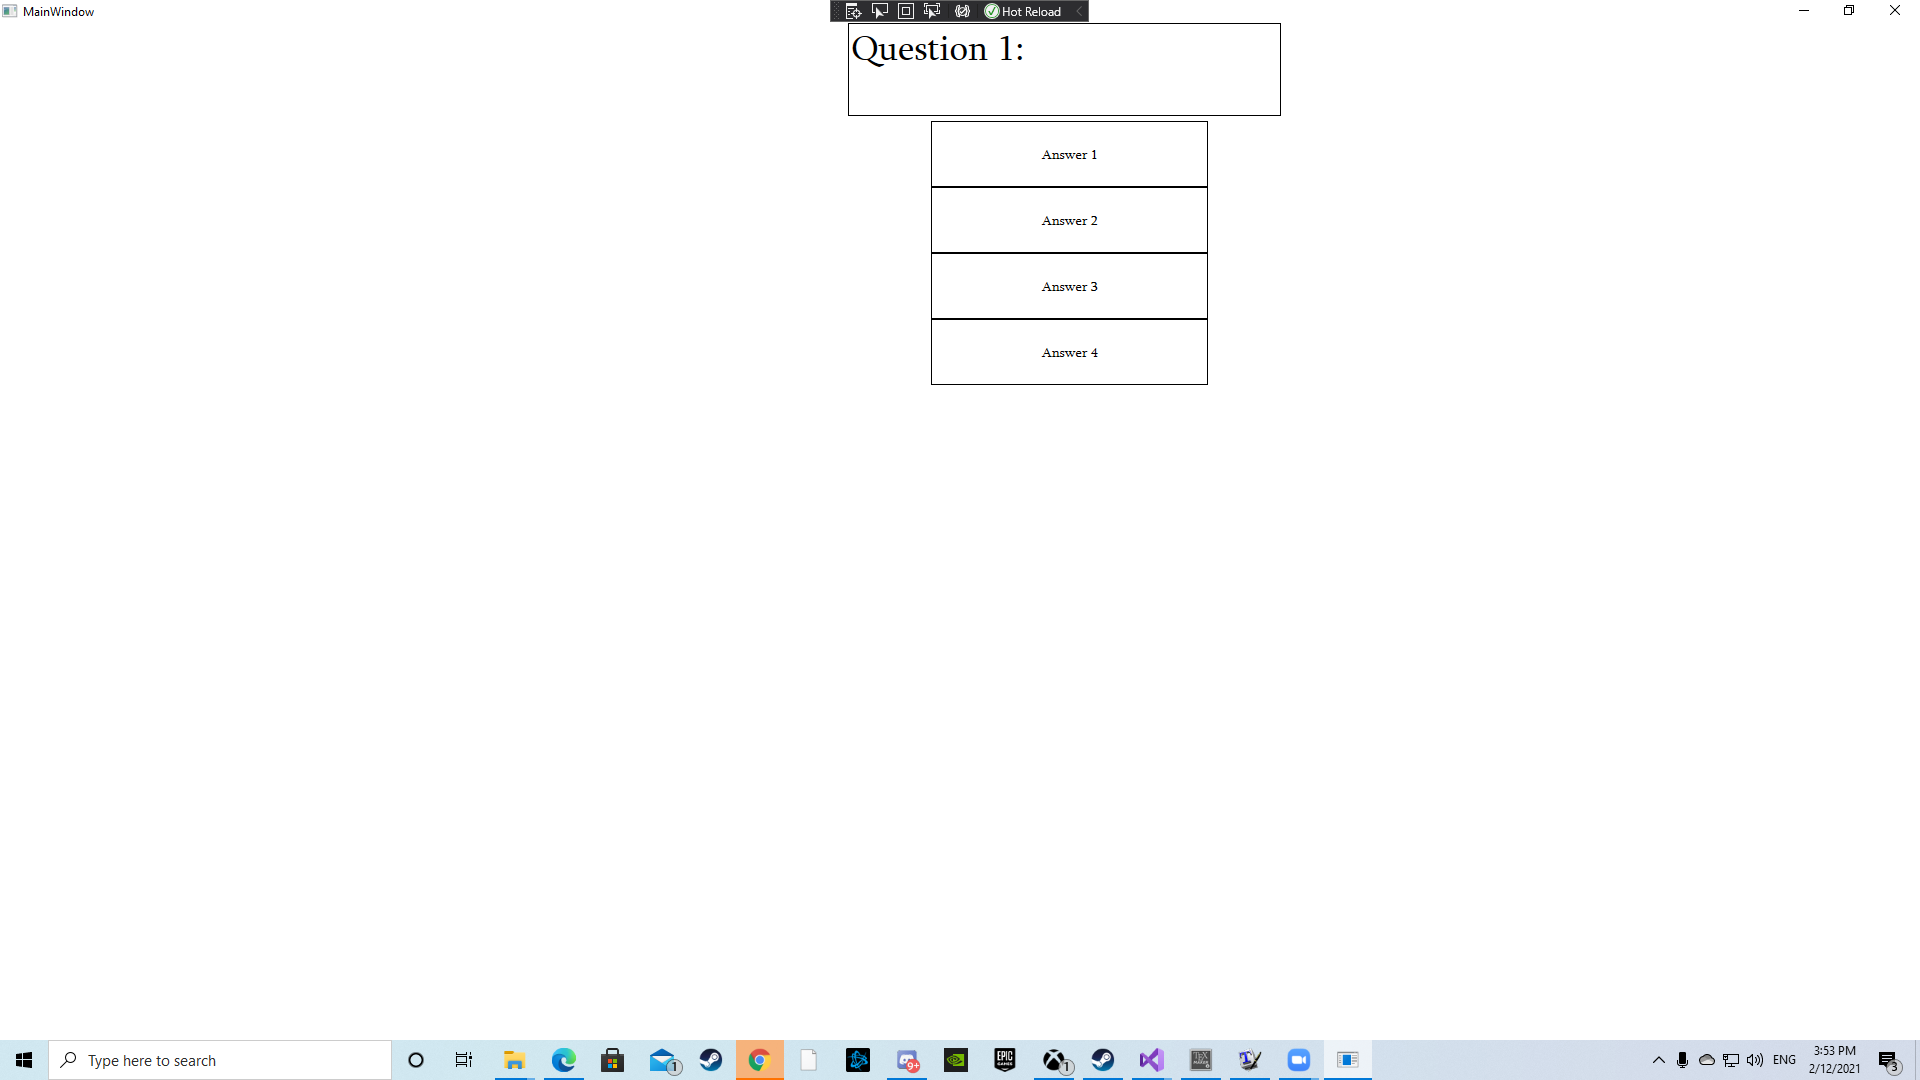
\includegraphics[height=150px, width=250px]{Interface1.png}
\caption{Interface 1}
\label{Interface1}
\end{figure}
\begin{figure}[ht!]
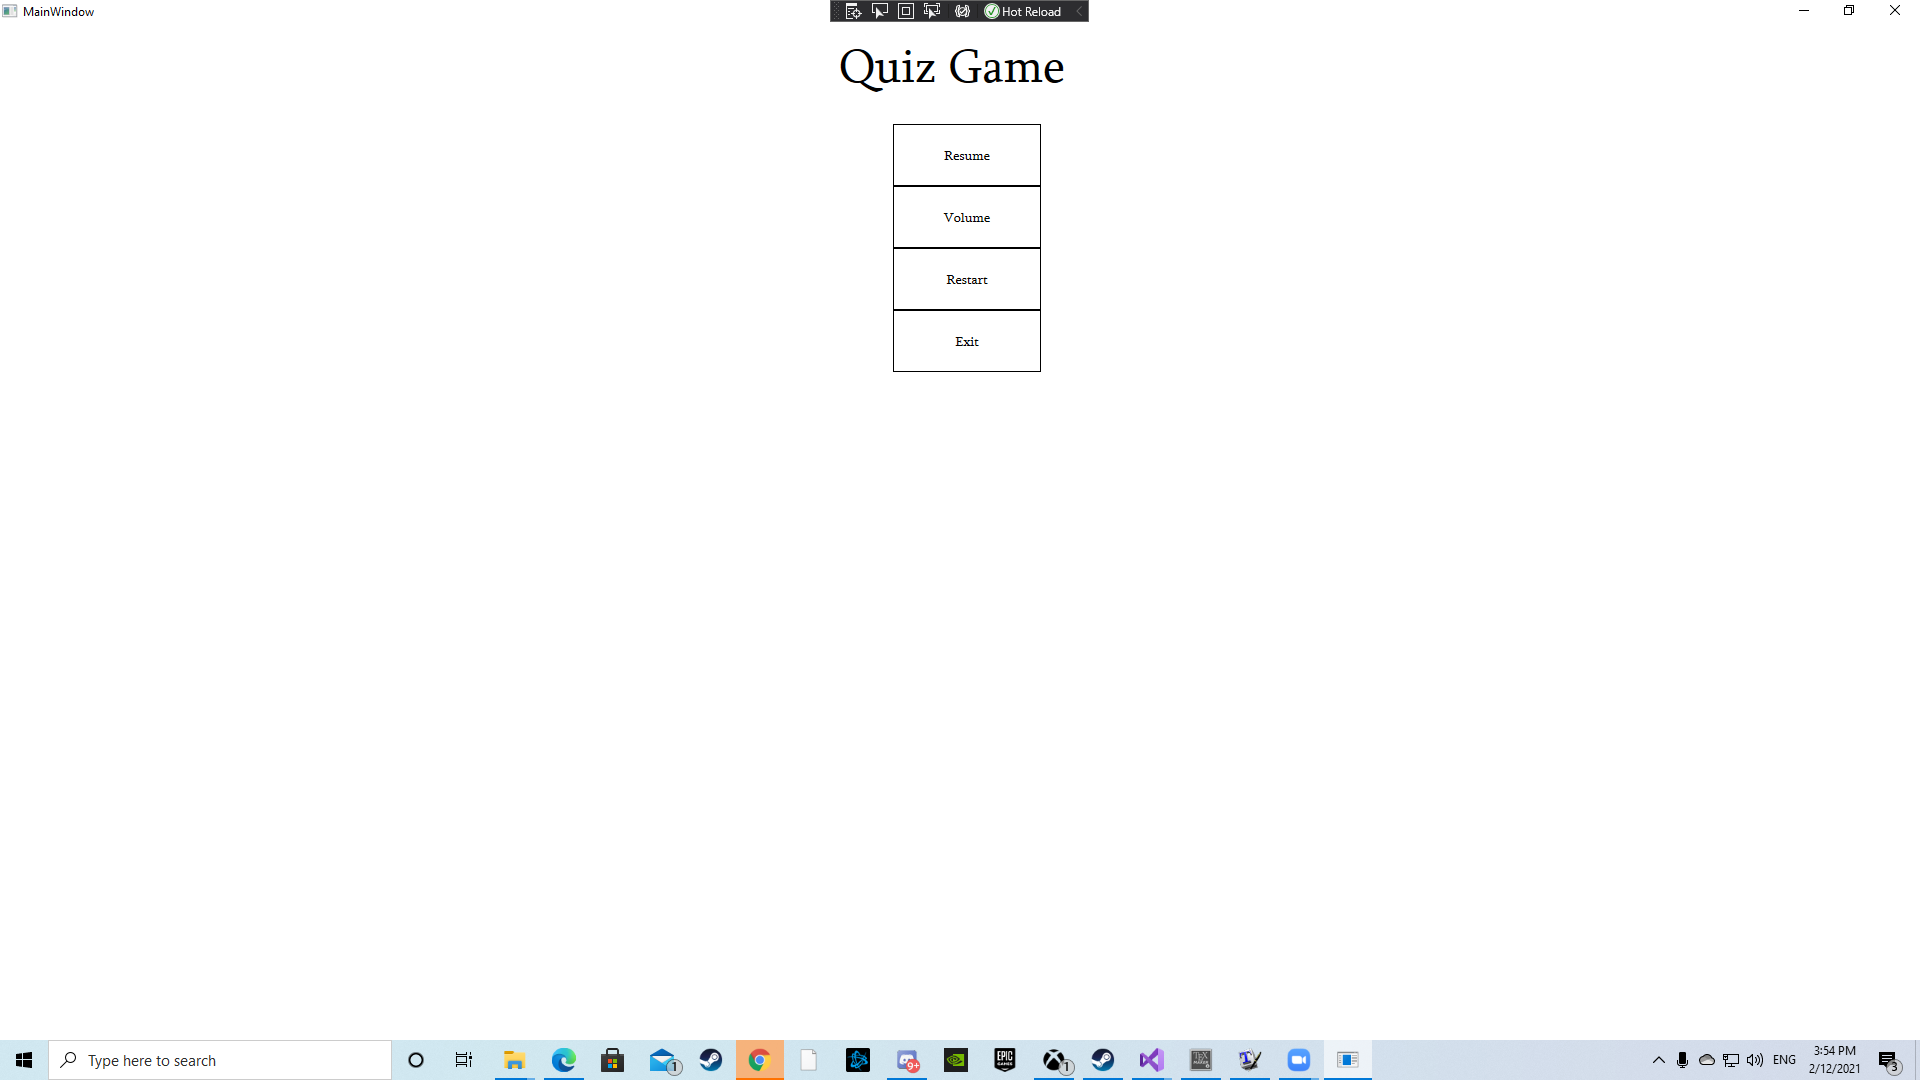
\includegraphics[height=150px, width=250px]{Interface2.png}
\caption{}
\label{Interface1}
\end{figure}
\begin{figure}[ht!]
\includegraphics[height=150px, width=250px]{interface3.png}
\caption{start menu}
\label{Interface1}
\end{figure}



\section{Project Timeline}
\begin{itemize}
\item Project Proposal Draft 02/01/2021: We got the basics of the project with topic and general idea. Also some of the features it will have.
\item Project Proposal Update 02/12/2021: We updated the non functional and functional aspects. We also talked about use cases and requirements.
Project Interface presentation 2/16/2021: We talked  briefly  about the overview of the project and looked at the interface mock ups. Dr. Guerin gave us feedback and some ideas for the project.
\item Project Update 4 3/19/2021: We have started on the structure and project time line.We have also started a UML following the project on the project structure section.
\item Interfaces and Elements 04/01/2021: We will have most of the interfaces and elements ready.
\item Database 04/06/2021: The database will be ready for use.
\item Finished 04/20/2021: The product is finished and ready to be demoed.
\end{itemize}
 
\section{Project Structure}
 	The project will have default question that will be loaded into a data base.
The database is set up to have categorizes organized under an ID.It would be connected to a questions table.The table would have a topic ID,and the actual question.The answers table would have a question ID to know which questions to go to.It would also have a answer section to hold the answers,and a correct field to see if they are correct.The Quiz bridge would organize the questions together for a quiz table.The quiz table would just have the name and the ID which would connect to the quiz ID in the bridge.

 	The GUI is set up at the Main menu  then allows you to go to settings,start menu,make quiz and quit. The start menu allows you to choose what type of quiz you would like and then allows you to start the game. Then each of the pages has option to go back to the main menu.The settings tab has the options to allows you to have a light mode, dark mode, and a mute button. The quiz interface has a text box that has a question on it,and buttons that have answers on it.

 	Users will be able to add questions at a later date  There will be about 4 categories to choose from to make the quiz on.There There will be options to change how the quizzes look to get an example of abstract factory. The main menu will have options to start, settings, create, and exit.The start menu will have categories and difficulties to choose from.There is also a random quiz option.

\subsection{UML Outline}
The UML starts in the Flazz Game class. If then leads to the settings class which has an option to change how the window looks.which leads to a interface for those two classes.The start menu class has options for choosing categories, going back to the main menu, making a random quiz,and starting a quiz.The categories class gives you a list of categories to choose from. At the end of quiz there is a score class which shows score. It also  gives you the option to quit or return to main menu.
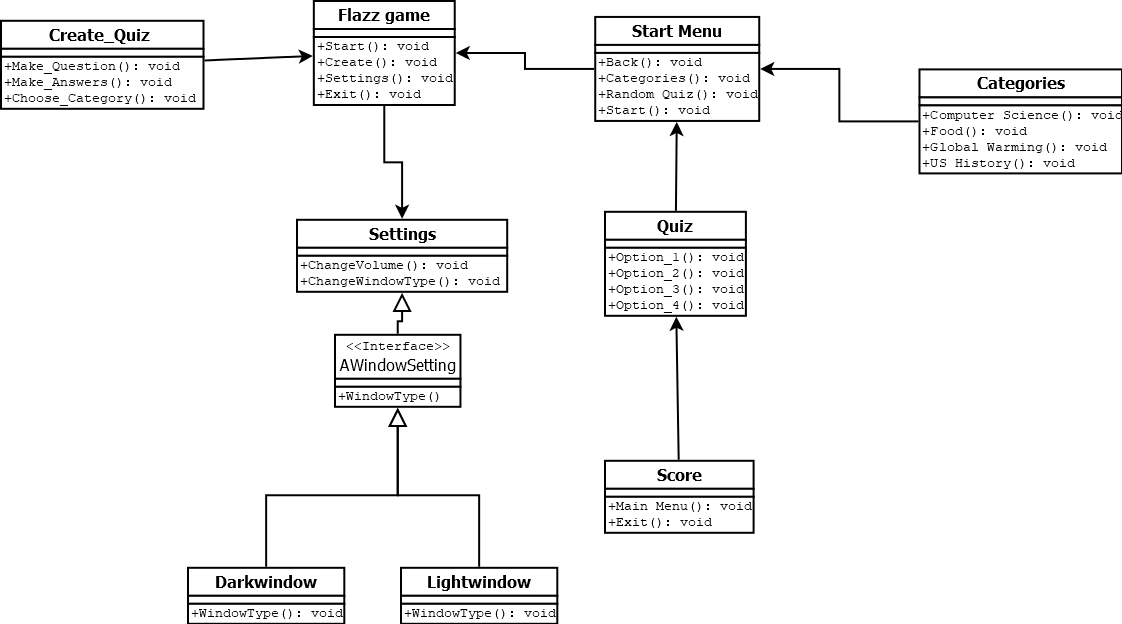
\includegraphics[height=300px, width=500px]{Flazz Game1.png}






\subsection{Design Patterns Used}
One of the patterns that is going to be used is the abstract factory method. It will be a light and dark mode for the windows. It will be found in the settings menu in the program.
The other design pattern will be the composite pattern. It will deal with the buttons and how they work on the quiz since clicking one will affect all of them in some way.
%Make sure to actually use at least 2 design patterns from this class.  This is not normally part of such documentation, but largely just specific to this class -- I want to see you use the patterns!%


\section{Results}
The project has most of the GUI done the database is almost done. All that needs to be done is allow the user to make a quiz and hook up the data base to the quiz section of the project. Most of the questions for the quizzes were added to the database. We lowered the amount of categorizes and removed difficulty. 
%This section will start out a little vague, but it should grow as your project evolves.  With each deliverable you hand in, give me a final summary of where your project stands.  By the end, this should be a reflective section discussing how many of your original goals you managed to attain/how many desired use cases you implemented/how many extra features you added.%

\subsection{Future Work}
The next thing we are doing with the project is finishing up the database, and adding the logic so it will display the quiz.The program will need to add the ability for a user to add a your own quiz.Then add a random quiz function if we have the time.
%Where are you going next with your project?
%For early deliverables, what are your next steps?  (HINT: you will typically want to look back at your timeline and evaluate: did you meet your expected goals?  Are you ahead of schedule?  Did you decide to shift gears and implement a new feature?)
%By the end, what do you plan on doing with this project?  Will you try to sell it?  Set it on fire?  Link to it on your resume and forget it exists?%




\begin{thebibliography}{1}

\bibitem{IEEEhowto:kopka}
H.~Kopka and P.~W. Daly, \emph{A Guide to \LaTeX}, 3rd~ed.\hskip 1em plus
  0.5em minus 0.4em\relax Harlow, England: Addison-Wesley, 1999.

\end{thebibliography}



\begin{IEEEbiography}{Michael Shell}
Biography text here.
\end{IEEEbiography}

% if you will not have a photo at all:
\begin{IEEEbiographynophoto}{John Doe}
Biography text here.
\end{IEEEbiographynophoto}

% insert where needed to balance the two columns on the last page with
% biographies
%\newpage

\begin{IEEEbiographynophoto}{Jane Doe}
Biography text here.
\end{IEEEbiographynophoto}





% that's all folks
\end{document}

